\documentclass{diploma}

\student{Мезенин Олег Александрович}
\group{М8О-406Б-21}
\theme{Проектирование системы переноса и генерации взаимосвязанных данных из производственной среды при тестировании образовательной платформы}

\supervisor{Миронов Евгений Сергеевич}
\firstConsultant{Ляпина Светлана Юрьевна}
\secondConsultant{---}
\reviewer{---}

\faculty{№ 8 <<Компьютерные науки и прикладная математика>>}
\department{806}
\speciality{01.03.02 <<Прикладная математика и информатика>>}
\profile{Информатика}

% Здесь необходим разрыв строки из-за особенностей титульной страницы
\departmentFullName{№ 806}
\headOfDepartment{Крылов Сергей Сергеевич}

% Дата. Оставляем пустое место для дня
\date{\uline{\hspace{24pt}} мая \the\year\ года}

\newglossaryentry{data-transfer}{
    name={Перенос данных},
    description={это процесс копирования и перемещения данных из одного источника или системы в другую без удаления данных из оригинальной базы данных}
}

\newacronym{db}{БД}{база данных}

\newacronym{dbms}{СУБД}{система управления базами данных}

\newacronym{software}{ПО}{программное обеспечение}


\addbibresource{main.bib}

% Иллюстрации всегда по центру
\makeatletter
\g@addto@macro\@floatboxreset\centering
\makeatother

% Настройки для листинга
\lstset{
  literate={:=}{{$\gets$}}1 {<=}{{$\leq$}}1 {>=}{{$\geq$}}1 {!=}{{$\neq$}}1 {\{\}}{{$\emptyset$}}1 {NOTIN}{{$\notin$}}1 {\#}{{$\rhd$}}1,
  keywordstyle=\color{black}\bfseries,
  basicstyle=\ttfamily\small,
  morekeywords={if, then, else, endif, while, do, end, for, each, in, return, to},
}
    
\begin{document}
\maketitle

% \includepdf[pages=-]{extra/task} % Задание
\setcounter{page}{2} % Устанавливает счётчик страниц

\abstract % Структурный элемент: РЕФЕРАТ

\keywords{БАЗЫ ДАННЫХ, ПЕРЕНОС ВЗАИМОСВЯЗАННЫХ ДАННЫХ, ТЕСТИРОВАНИЕ ОБРАЗОВАТЕЛЬНОЙ ПЛАТФОРМЫ, POSTGRESQL, ГЕНЕРАЦИЯ ДАННЫХ}

В выпускной квалификационной работе бакалавра была спроектирована система переноса и генерации взаимосвязанных данных при тестировании образовательной платформы. Разработаны алгоритмы переноса и генерации взаимосвязанных данных, создана грамматика языка для описания входных данных. Был разработан и протестирован прототип системы, позволяющий переносить данные, и был проведён анализ жизнеспособности системы.

Систему можно использовать при тестировании программных продуктов любой сферы деятельности.
 % Реферат

\tableofcontents % Содержание 
\termsanddefenitions % Термины и определения
\listofabbreviations % Перечень сокращений и обозначений

\introduction % Структурный элемент: ВВЕДЕНИЕ

В настоящее время рынок онлайн-образования демонстрирует значительный рост: объём российского рынка образовательных технологий в 2024 году составил 149 миллиардов рублей, увеличившись на 21\% по сравнению с 2023 годом \cite{online-edu}. Сегмент онлайн-образования, направленный на детей, составляет 29\% \cite{online-edu-child}. В связи с этим внимание следует уделить платформам, предназначенным для участников средней общеобразовательной школы.

Эти платформы требуют надёжной системы управления данными для обеспечения стабильной работы и поддержки большого количества пользователей. Одним из распространённых решений в области управления базами данных является PostgreSQL~\cite{postgresql} — реляционная система управления базами данных с открытым исходным кодом.

В процессе разработки платформы важно уделять особое внимание качеству и надёжности. Это делает тестирование незаменимой стадией разработки. Благодаря тестированию можно убедиться в стабильности и бесперебойной работе систем.

Использование реальных данных и проведение тестов в производственной среде позволяет максимально точно оценить работоспособность системы. Но такой подход сопряжён с рисками, такими как нарушения конфиденциальности данных и потенциальные сбои в работе системы.

Чтобы тестирование образовательных платформ было безопасным и в то же время позволяло бы максимально точно оценить работоспособность системы, необходимо создать тестовую среду, максимально приближенную к производственным условиям. Создание тестовой среды требует тщательной проработки и учёта всех аспектов, связанных с функционированием платформы. Это включает в себя настройку инфраструктуры, идентичной производственной, и воспроизведение всех взаимосвязей данных, которые присутствуют в реальных условиях эксплуатации.

Особую значимость в этом контексте приобретает работа с данными. Для достижения максимальной схожести с производственной средой необходимо использовать тестовые данные, которые точно отражают объёмы, структуры и взаимосвязи данных, присутствующие в реальной системе.

Создание тестового набора данных может быть реализовано с использованием различных методик. Один из подходов включает полный перенос данных из производственной базы данных с последующей анонимизацией конфиденциальной информации. Утилита pg\_dump~\cite{pg-dump} может быть использована для экспорта данных из PostgreSQL, обеспечивая перенос структуры и содержимого базы данных.

Для защиты пользовательской информации и анонимизации данных можно применить утилиту pg\_anonymizer~\cite{pg-anonymizer}, которая помогает скрыть чувствительные данные, заменяя их на фиктивные значения, что сохраняет конфиденциальность пользователей.

Основной недостаток данного метода заключается в невысокой скорости переноса всех данных, что может быть критичным при работе с крупными наборами данных и требовать значительных временных затрат для выполнения всей операции.

Частичный перенос данных может быть более подходящим для тестирования, так как зачастую не требуется полный объём данных для покрытия большинства сценариев. Но этот подход сопряжён с рядом вопросов и потенциальных сложностей, которые опишем ниже.

При полном переносе данных тестировщик получает доступ ко всем данным, что позволяет ему проводить тестовые сценарии. В случае частичного переноса данных требуется определить и описать необходимые для тестирования данные, избегая глубокого изучения структуры базы данных и её связей. Возникает вопрос, каким образом тестировщику описать данные, нужные для проведения тестов.

Следующим вопросом является сохранение целостности данных. В случае полного переноса реляционная целостность поддерживается автоматически, поскольку все взаимосвязанные данные переносятся полностью, обеспечивая корректность и согласованность системы. При частичном переносе необходимо уделить особое внимание поддержанию целостности данных. Недопустимо, чтобы после переноса в тестовой среде данных было недостаточно для выполнения тестовых сценариев. Следовательно, второй вопрос заключается в обеспечении целостности данных при минимизации объёма переносимых данных.

Перенос данных из производственной среды с использованием анонимизации представляет собой лишь один из способов получения тестовых данных. Альтернативный подход состоит в генерации данных на основе заданных характеристик. Этот процесс может выглядеть следующим образом. Пользователь задаёт параметры, которые могут сопровождаться набором или диапазоном значений. Затем программа генерирует тестовые данные, основываясь на фактических данных, либо на схеме данных производственной базы, а также на указанных пользователем характеристиках. Таким образом, полученные данные будут иметь структуру, аналогичную реальным данным, но не будут связаны с конкретными записями в производственной базе. Но для этого метода возникают вопросы описания пользователем необходимых данных и их корректной генерации.

Дипломная работа будет посвящена проектированию системы, которая должна поддерживать следующую функциональность:
\begin{itemize}
    \item перенос взаимосвязанных данных из одной базы данных в другую с применением методов анонимизации,
    \item генерацию тестовых данных.
\end{itemize}
В рамках работы будут рассмотрены алгоритмы переноса и генерации данных. Также будет разработан язык для описания данных и прототип системы.
 % Введение

\section{Постановка задачи и теоретические предпосылки}

\subsection{Тестирование}

Чтобы определить требования к нашей системе, для начала нужно разобраться с основными аспектами тестирования программного обеспечения.

\subsubsection{Процесс тестирования}

Тестирование — это процесс оценки системы или её компонентов с целью проверки их соответствия заданным требованиям. Основная цель тестирования заключается в выявлении дефектов, обеспечении качества и подтверждении работоспособности программного обеспечения.

Процесс тестирования можно разбить на несколько ключевых этапов~\cite{rex-black}:

\begin{enumerate}
    \item Планирование:
    \begin{itemize}
        \item разрабатывается стратегия тестирования, включая выбор типов тестирования;
        \item создается тест-план, где описываются ресурсы, сроки, и критерии начала и завершения тестирования;
        \item проводится анализ рисков, связанных с тестированием и определяются действия для минимизации их воздействия.
    \end{itemize}

    \item Подготовка:
    \begin{itemize}
        \item разработка тестовых случаев и сценариев на основе требований и спецификаций;
        \item подготовка тестовой среды, включая оборудование и программные средства, необходимые для проведения тестов;
        \item подготовка данных для тестирования и настройка автоматизированных тестов, если они предусмотрены.
    \end{itemize}

    \item Проведение:
    \begin{itemize}
        \item непосредственное выполнение тестов согласно плану тестирования;
        \item фиксация и документирование результатов тестирования, выявление дефектов и несоответствий.
    \end{itemize}

    \item Совершенствование:
    \begin{itemize}
        \item анализ результатов тестирования и составление отчёта по итогам выполненной работы;
        \item обмен опытом и полученными знаниями внутри команды и с другими заинтересованными сторонами;
        \item обновление и улучшение тестовых документов и процессов на основе полученных данных.
    \end{itemize}
\end{enumerate}

Наша система будет применяться на этапе подготовки: с её помощью можно будет создавать тестовые данные.

\subsection{Ручное и автоматизированное тестирование}

Тестирование можно классифицировать на ручное и автоматизированное.

Ручное тестирование предполагает процесс, при котором тестировщик выполняет тесты без помощи автоматизированных инструментов.
Оно позволяет глубже вникнуть в пользовательский опыт, и его легко применять к новым или часто изменяющимся функциональностям, однако оно может быть времяемким, подвержено человеческим ошибкам и не всегда позволяет повторить результаты для их сравнения.

Автоматизированное тестирование предполагает использование программных инструментов для автоматизации выполнения тестовых сценариев. Это предполагает разработку скриптов, которые автоматически выполняют тесты и сверяют результаты с ожидаемыми.
Автоматизированное тестирование обеспечивает высокую скорость и стабильность результатов, что делает его эффективным для регрессионного тестирования и стабильных функциональностей, однако требует значительных ресурсов для разработки скриптов и не всегда подходит для тестирования пользовательских интерфейсов и динамически изменяющихся требований.

Оба подхода часто используются совместно для достижения наилучшего результата. Обычно ручное тестирование применяют на начальных стадиях или для исследовательского тестирования, тогда как автоматизированное тестирование использует для повторяющихся задач или сложных сценариев, которые требуют стабильного выполнения.

\subsection{Сценарии использования}

Перед определением требований к нашей системы рассмотрим возможные сценарии использования.

Определим роли:

\begin{itemize}
    \item тестировщик — специалист, занимающийся проверкой качественности, надёжности и работоспособности программного обеспечения;
    \item разработчик — специалист, занимающийся разработкой программного обеспечения;
    \item DevOps-инженер — специалист, занимающийся поддержкой процессов CI/CD.
\end{itemize}

Будем называть метаданными входные данные, включающие в себя правила переноса, генерации или анонимизации данных.

\subsubsection{Перенос данных для проведения тестовых сценариев}

\underline{Роли}:

\begin{itemize}
    \item тестировщик;
    \item разработчик.
\end{itemize}

\underline{Цель}: создать тестовые данные на основе существующих реальных данных для их дальнейшего применения в тестовых сценариях.

\underline{Предпосылки}:

\begin{itemize}
    \item разработчиком написаны метаданные, включающие в себя правила переноса и анонимизации данных;
    \item тестировщик осведомлен о метаданных, необходимых для проведения тестовых сценариев;
    \item тестировщик имеет уникальный идентификатор исходной базы данных;
    \item имеется пустая тестовая база данных, доступ к которой имеется у тестировщика.
\end{itemize}

\underline{Основной сценарий}:

\begin{enumerate}
    \item Тестировщик осуществляет изменения в метаданных при необходимости.
    \item Тестировщик инициирует запуск CLI, указывая следующие параметры:
    \begin{itemize}
        \item уникальный идентификатор исходной базы;
        \item уникальный идентификатор целевой базы или параметры подключения к ней;
        \item метаданные или уникальный идентификатор метаданных.
    \end{itemize}
    \item Тестировщик ожидает завершения процесса переноса данных.
\end{enumerate}

\underline{Постусловия}:

\begin{itemize}
    \item тестировщик применяет данные, сгенерированные на основе реальных данных, в тестовых сценариях.
\end{itemize}

\underline{Исключения}:

\begin{itemize}
    \item тестировщик получает ошибку некорректных метаданных, если он менял их, после пункта б.
\end{itemize}


\subsubsection{Диагностика ошибки}

\underline{Роли}:

\begin{itemize}
    \item тестировщик.
\end{itemize}

\underline{Цель}: провести диагностику ошибки, возникшей с определенными данными в продуктивной среде.

\underline{Предпосылки}:

\begin{itemize}
    \item в продуктивной среде обнаружены проблемы с определенными данными, такими как данные пользователя;
    \item тестировщик владеет уникальным идентификатором данных, в которых выявлена ошибка в продуктивной среде;
    \item тестировщик имеет уникальный идентификатор исходной базы данных;
    \item имеется пустая тестовая база данных, доступ к которой имеется у тестировщика.
\end{itemize}

\underline{Основной сценарий}:

\begin{enumerate}
    \item Тестировщик описывает метаданные, включая данные, в которых произошла ошибка.
    \item Тестировщик инициирует запуск CLI, указывая следующие параметры:
    \begin{itemize}
        \item уникальный идентификатор исходной базы;
        \item уникальный идентификатор целевой базы или параметры подключения к ней;
        \item метаданные.
    \end{itemize}
    \item Тестировщик ожидает завершения процесса переноса данных.
\end{enumerate}

\underline{Альтернативный сценарий}:

\begin{itemize}
    \item тестировщик может взять готовые метаданные, если они ему подходит, а не описывать свои.
\end{itemize}

\underline{Постусловия}:

\begin{itemize}
    \item тестировщик осуществляет взаимодействие с перенесенными данными и проводит диагностику ошибки.
\end{itemize}

\underline{Исключения}:

\begin{itemize}
    \item тестировщик получает ошибку некорректных метаданных после пункта б.
\end{itemize}


\subsubsection{Тестирование новой миграции}

\underline{Роли}:

\begin{itemize}
    \item тестировщик;
    \item разработчик.
\end{itemize}

\underline{Цель}: провести тестирование новой миграции.

\underline{Предпосылки}:

\begin{itemize}
    \item тестировщик имеет уникальный идентификатор исходной базы данных;
    \item имеется пустая тестовая база данных, доступ к которой имеется у тестировщика;
    \item разработчик создал новую миграцию, нуждающуюся в тестировании;
    \item разработчик предоставил метаданные к миграции, содержащие правила анонимизации и переноса данных.
\end{itemize}

\underline{Основной сценарий}:

\begin{enumerate}
    \item Тестировщик инициирует запуск CLI, указывая следующие параметры:
    \begin{itemize}
        \item уникальный идентификатор исходной базы;
        \item уникальный идентификатор целевой базы или параметры подключения к ней;
        \item предоставленные метаданные.
    \end{itemize}
    \item Тестировщик ожидает завершения процесса переноса данных.
\end{enumerate}

\underline{Постусловия}:

\begin{itemize}
    \item тестировщик взаимодействует с перенесенными данными и осуществляет тестирование миграций.
\end{itemize}


\subsubsection{Перенос данных для автоматизированного тестирования}

\underline{Роли}:

\begin{itemize}
    \item тестировщик;
    \item разработчик;
    \item DevOps-инженер.
\end{itemize}

\underline{Цель}: обеспечеть возможность проведения автоматизированного тестирования изменений через сценарий CI/CD.

\underline{Предпосылки}:

\begin{itemize}
    \item разработчиком написаны метаданные, включающие в себя правила переноса и анонимизации данных;
    \item тестировщиком реализованы автоматизированные тесты;
    \item DevOps-инженер разработал сценарий CI/CD, который, в случае появления нового запроса на слияния в системе контроля версий, инициирует развёртывание тестового окружения с пустой базой данных и осуществляет перенос необходимых данных с помощью нашей системы.
\end{itemize}

\underline{Основной сценарий}:

\begin{enumerate}
    \item Разработчик вносит изменения в исходный код и создает новый запрос на слияние в системе контроля версий.
    \item Запускается процесс CI/CD, который выполняет следующие действия:
    \begin{itemize}
        \item развёртывание тестового окружения с пустой базой данных;
        \item перенос необходимых данных в тестовую базу с помощью нашей системы;
        \item автоматический запуск тестов для проверки корректности внесённых изменений.
    \end{itemize}
\end{enumerate}


\subsubsection{Генерация данных для проведения тестовых сценариев}

\underline{Роли}:

\begin{itemize}
    \item тестировщик;
    \item разработчик.
\end{itemize}

\underline{Цель}: создать тестовые данные на основе существующих реальных данных для их дальнейшего применения в тестовых сценариях.

\underline{Предпосылки}:

\begin{itemize}
    \item разработчиком написаны метаданные, включающие в себя правила генерации данных;
    \item тестировщик осведомлен о метаданных, необходимых для проведения тестовых сценариев;
    \item тестировщик имеет уникальный идентификатор исходной базы данных;
    \item имеется пустая тестовая база данных, доступ к которой имеется у тестировщика.
\end{itemize}

\underline{Основной сценарий}:

\begin{enumerate}
    \item Тестировщик осуществляет изменения в метаданных при необходимости.
    \item Тестировщик инициирует запуск CLI, указывая следующие параметры:
    \begin{itemize}
        \item уникальный идентификатор исходной базы;
        \item уникальный идентификатор целевой базы или параметры подключения к ней;
        \item метаданные или уникальный идентификатор метаданных.
    \end{itemize}
    \item Тестировщик ожидает завершения процесса генерации данных.
\end{enumerate}

\underline{Постусловия}:

\begin{itemize}
    \item тестировщик применяет сгенерированные данные в тестовых сценариях.
\end{itemize}

\underline{Исключения}:

\begin{itemize}
    \item тестировщик получает ошибку некорректных метаданных, если он менял их, после пункта б.
\end{itemize}


\subsection{Определение требований к системе}

Требования к системе можно классифицировать на две основные категории: функциональные и архитектурные. Функциональные требования описывают конкретный набор функций и возможностей, которые система должна обеспечивать для удовлетворения потребностей пользователей. Требования к свойствам архитектуры системы фокусируются на качественных характеристиках системы, которые обеспечивают её устойчивую и эффективную работу.

\subsubsection{Функциональные требования}

Система должна поддерживать следующий функционал:

\begin{itemize}
    \item Перенос и анонимизация данных. Система должна обеспечивать возможность переноса взаимосвязанных данных между базами данных, а также их анонимизацию. Правила выбора взаимосвязанных данных и правила анонимизации задаются метаданными.
    \item Генерация данных. Система должна предоставлять функционал для генерации данных. Правила генерации задаются метаданными.
    \item Работа с метаданными. Система должна осуществлять проверку корректности метаданных, а также обеспечивать функциональность для загрузки предварительно подготовленных метаданных или их интеграции на этапе ввода данных.
    \item Гибкость в выборе базы данных. Необходимо внедрить функциональность, позволяющую пользователю выбрать базу данных, указав как уникальный идентификатор базы, так и строку подключения.
\end{itemize}

\subsubsection{Требования к свойствам архитектуры}

Архитектура системы должна соответствовать следующим критериям:

\begin{itemize}
    \item Безопасность. Архитектура должна обеспечивать защиту от несанкционированного доступа к базе данных, а также обеспечивать защиту конфиденциальной информации.
    \item Надёжность. Система должна функционировать без сбоев в течение продолжительных периодов времени. Это предполагает наличие мер по обеспечению отказоустойчивости и возможности восстановления после сбоев.
    \item Высокая производительность. Архитектура должна обеспечивать эффективную обработку больших объёмов данных.
    \item Асинхронная обработка запросов. Поскольку перенос или генерация данных может занимать значительное время, система должна поддерживать выполнение запросов в асинхронном режиме. Это означает, что клиентские приложения не должны блокироваться в ожидании завершения операции, но должны иметь возможность проверять статус выполнения запроса по мере необходимости.
\end{itemize}

\section{Проектирование системы, разработка языка и алгоритма}

\subsection{Архитектура системы}

Рассмотрим архитектуру системы по модели С4~\cite{c4-model}.

\subsubsection{Взаимодействие систем}

\begin{figure}
  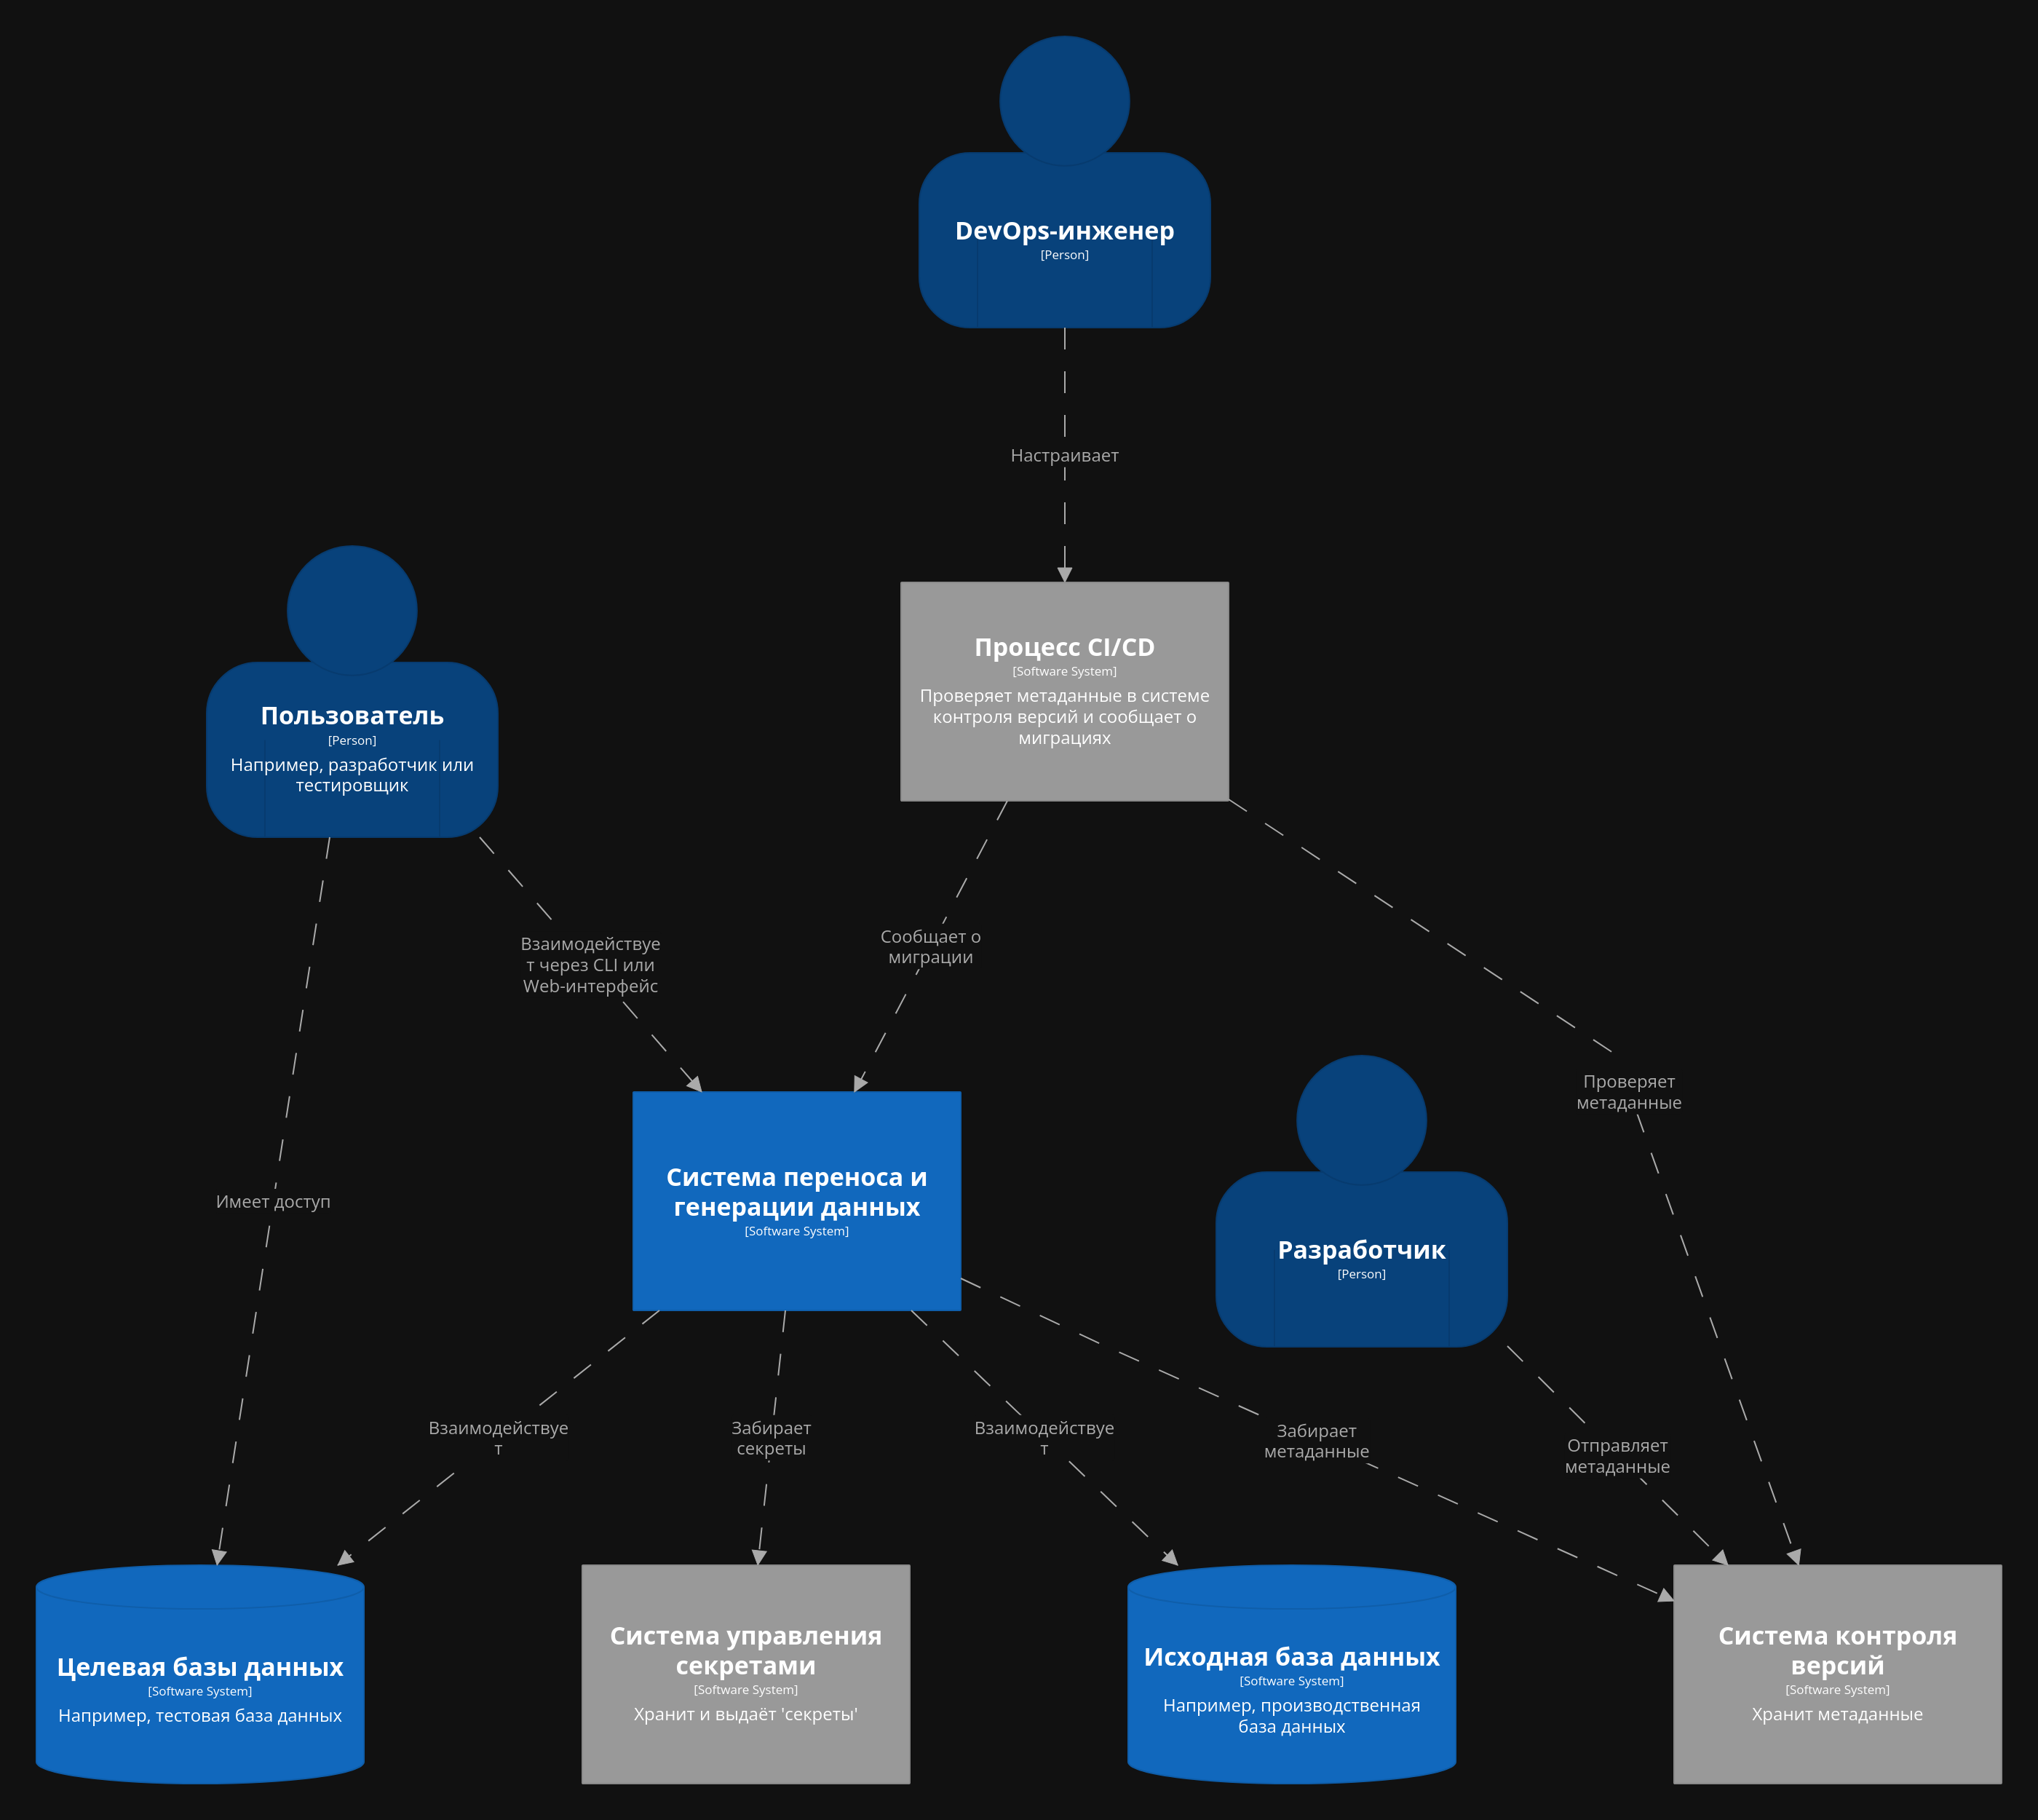
\includegraphics[scale=0.15]{./img/structurizr-SystemLandscape.png}
  \caption{Взаимодействие систем}
  \label{System Context}
\end{figure}

На уровне контекста можно наблюдать взаимодействие различных систем, а также взаимодействие этих систем с пользователями и специалистами.

Внешние системы выделены серым цветом:
\begin{itemize}
\item система контроля версий выступает в качестве хранилища метаданных, представленных разработчиком;
\item система управления секретами предоставляет данные для подключения к базе данных;
\item процесс CI/CD, который настраивает DevOps-инженер, выполняет несколько функций:
  \begin{itemize}
    \item генерация тестовой среды и запуск автоматизированных тестов при получении запроса на слияние в систему контроля версий;
    \item проверка корректности метаданных в момент их фиксации в системе контроля версий;
    \item при выполнении миграций осуществляется уведомление системы переноса и генерации данных о процессах миграции -- это необходимо для предотвращения неопределенного поведения, которое может возникнуть, если система в текущий момент работает с мигрируемой базой данных.
  \end{itemize}
\end{itemize}

Синим цветом выделены собственные системы: исходная и целевая базы данных, с которыми осуществляется взаимодействие пользователей, а также система переноса и генерации данных, которую мы рассмотрим более детально далее.

\subsubsection{Система переноса и генерации данных}

\begin{figure}
  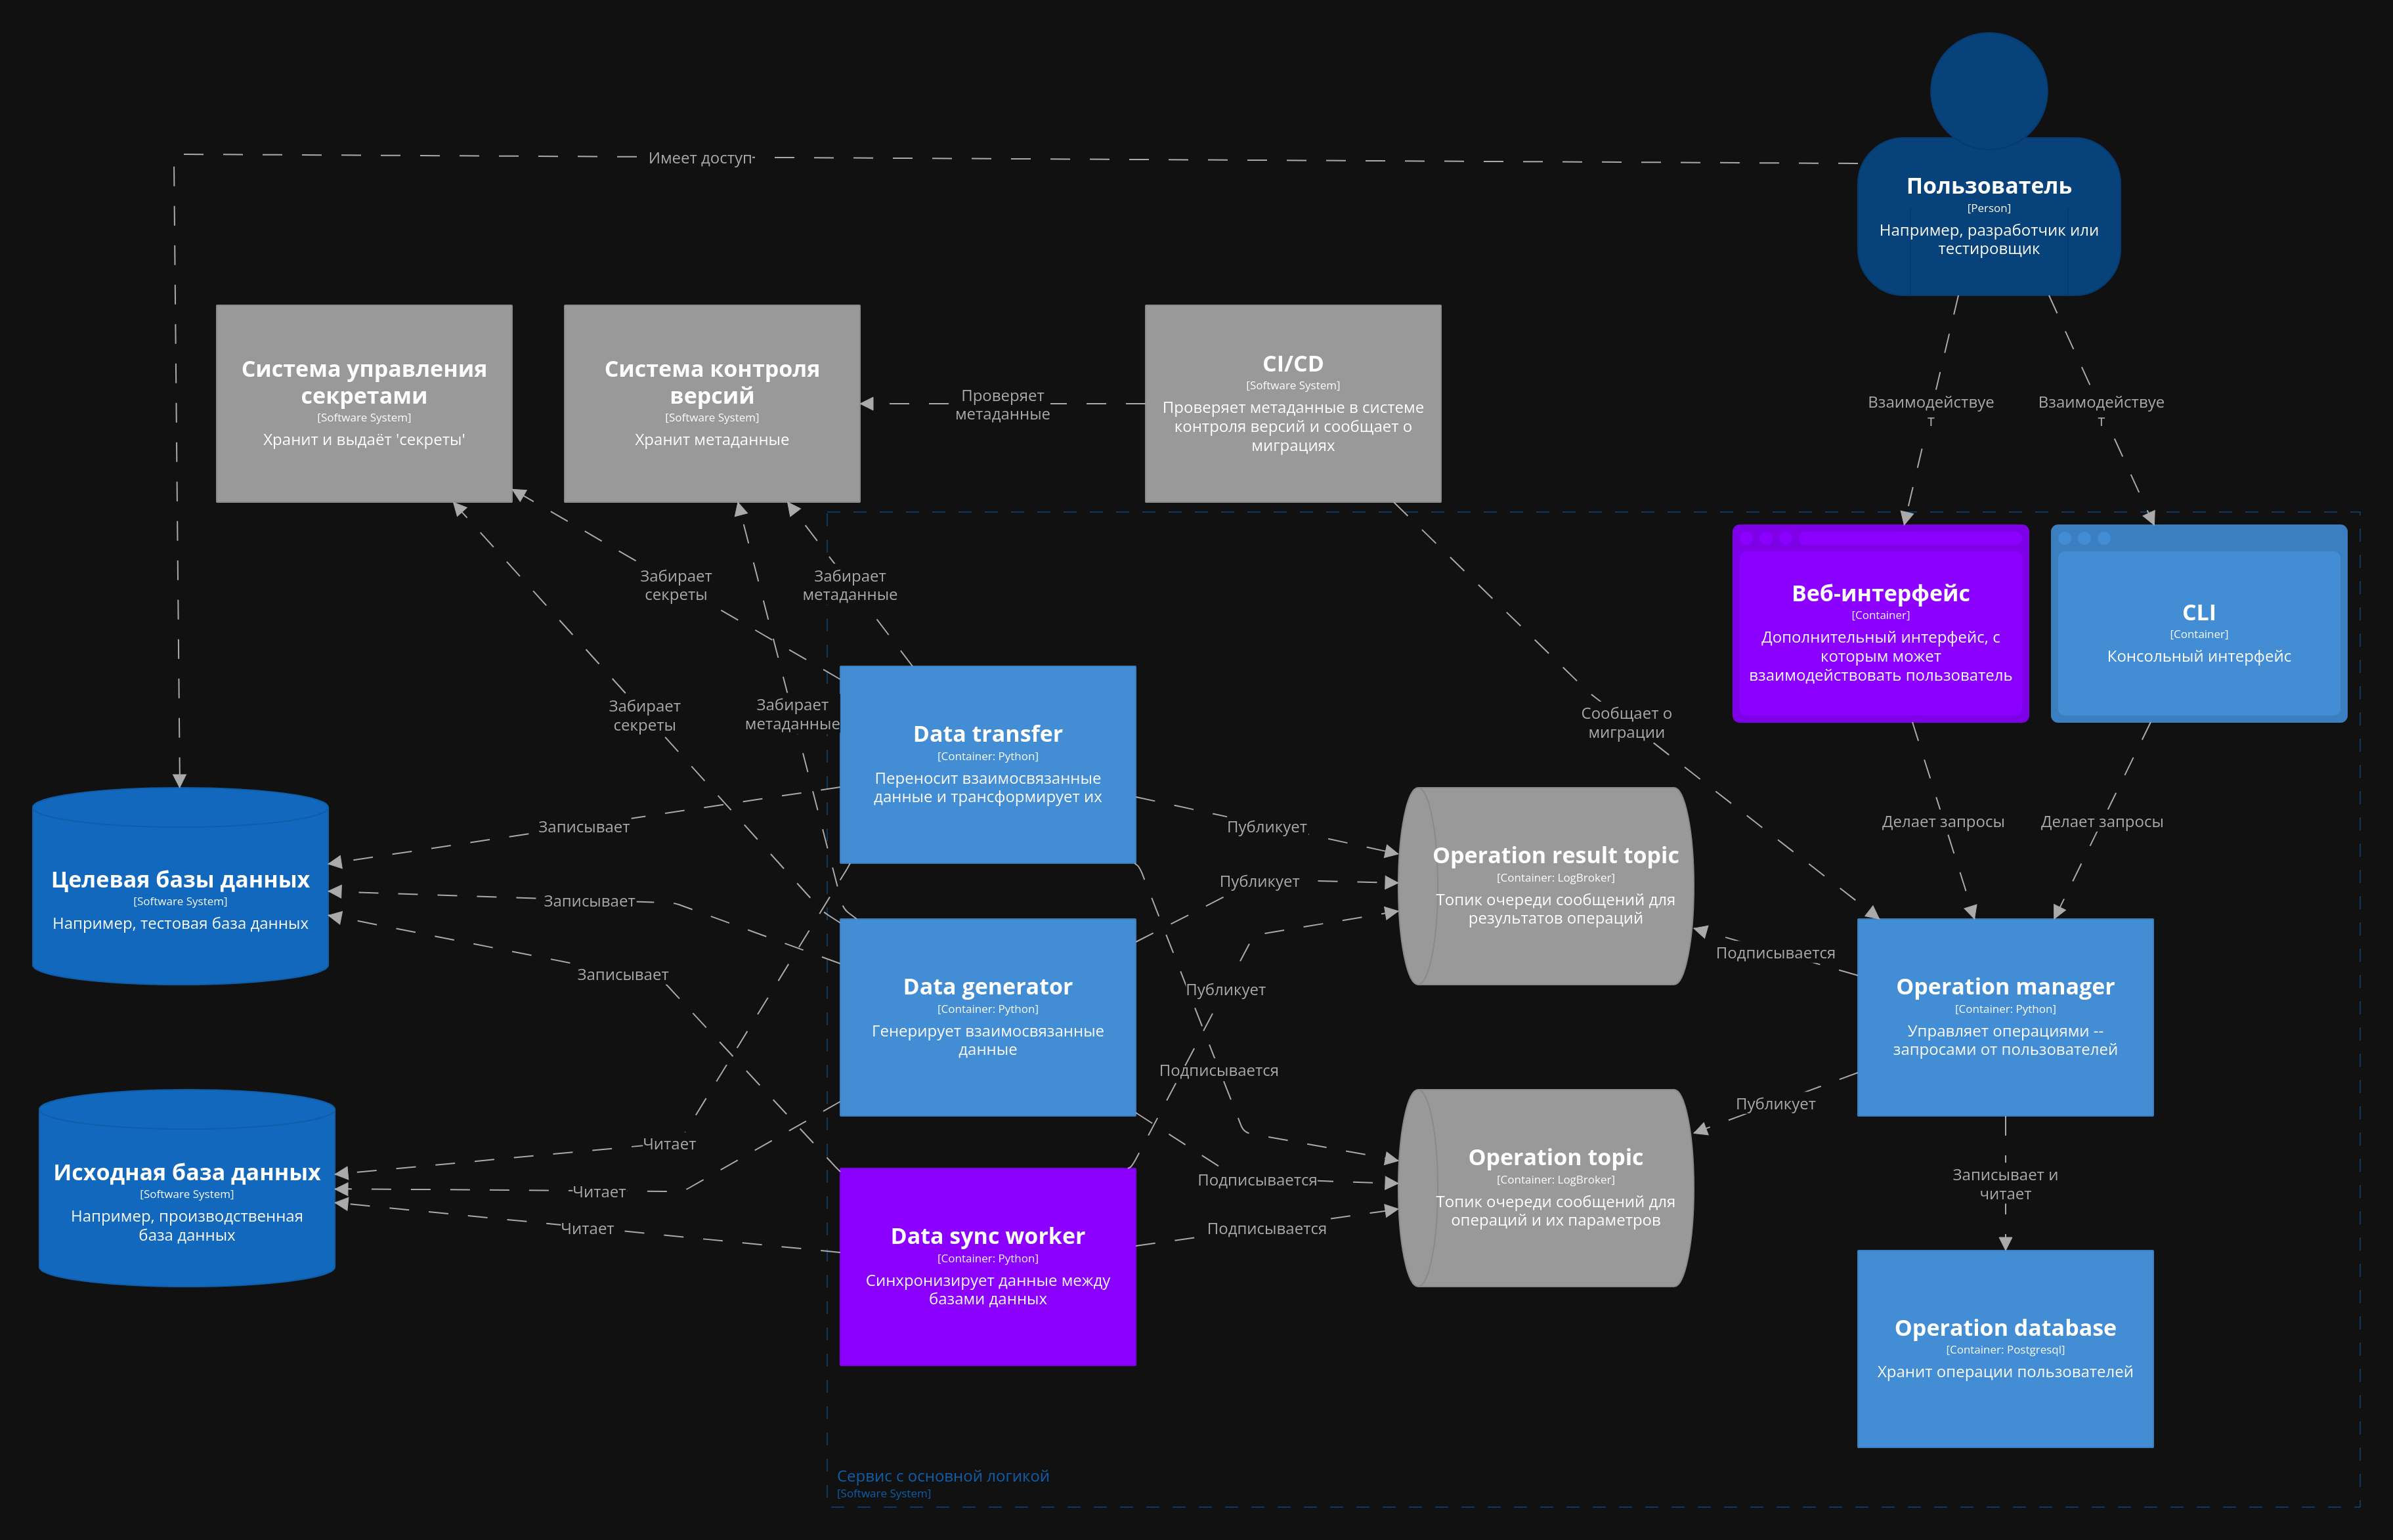
\includegraphics[scale=0.12]{./img/structurizr-Containers.png}
  \caption{Система переноса и генерации данных}
  \label{Containers}
\end{figure}

Рассмотрим систему переноса и генерации данных на уровне контейнеров.

Взаимодействие пользователя с системой осуществляется через командную строку (CLI), хотя может быть реализован и альтернативный интерфейс взаимодействия, например, веб-интерфейс (выделен фиолетовым как контейнер, который может быть добавлен в перспективе).

Пользователь посылает запросы в контейнер Operation Manager. Возможны два типа запросов: запуск операции по переносу или генерации данных, а также проверка статуса выполняемой операции. В случае получения запроса на запуск операции, информация об операции сохраняется в базе данных, а уникальный идентификатор операции возвращается пользователю, что позволяет ему отслеживать статус выполнения.

Далее Operation Manager отправляет запросы на выполнение операции в очередь сообщений Logbroker~\cite{logbroker}. Контейнер, обрабатывающий такой запрос, определяется типом операции: если речь идет о переносе данных, операция обрабатывается контейнером Data Transfer; если о генерации данных — контейнером Data Generator.

На схеме также представлен контейнер Data Sync Worker, являющийся гипотетическим контейнером, предназначенным для обработки операций по синхронизации данных в базах данных.

Контейнеры Data Transfer и Data Generator осуществляют перенос и генерацию данных, взаимодействуя с базами данных, системой контроля версий и системой управления секретами. В процессе выполнения операции, а также после её выполнения, информация о статусе возвращается в очередь сообщений, из которой Operation Manager извлекает данные и обновляет статус операции в базе данных.

Более детальное описание структуры компонентов Data Transfer и Data Generator будет представлено в последующих разделах.

Рассмотрим диаграмму последовательности взаимодействия пользователя с системой на примере генерации данных.

\begin{figure}
  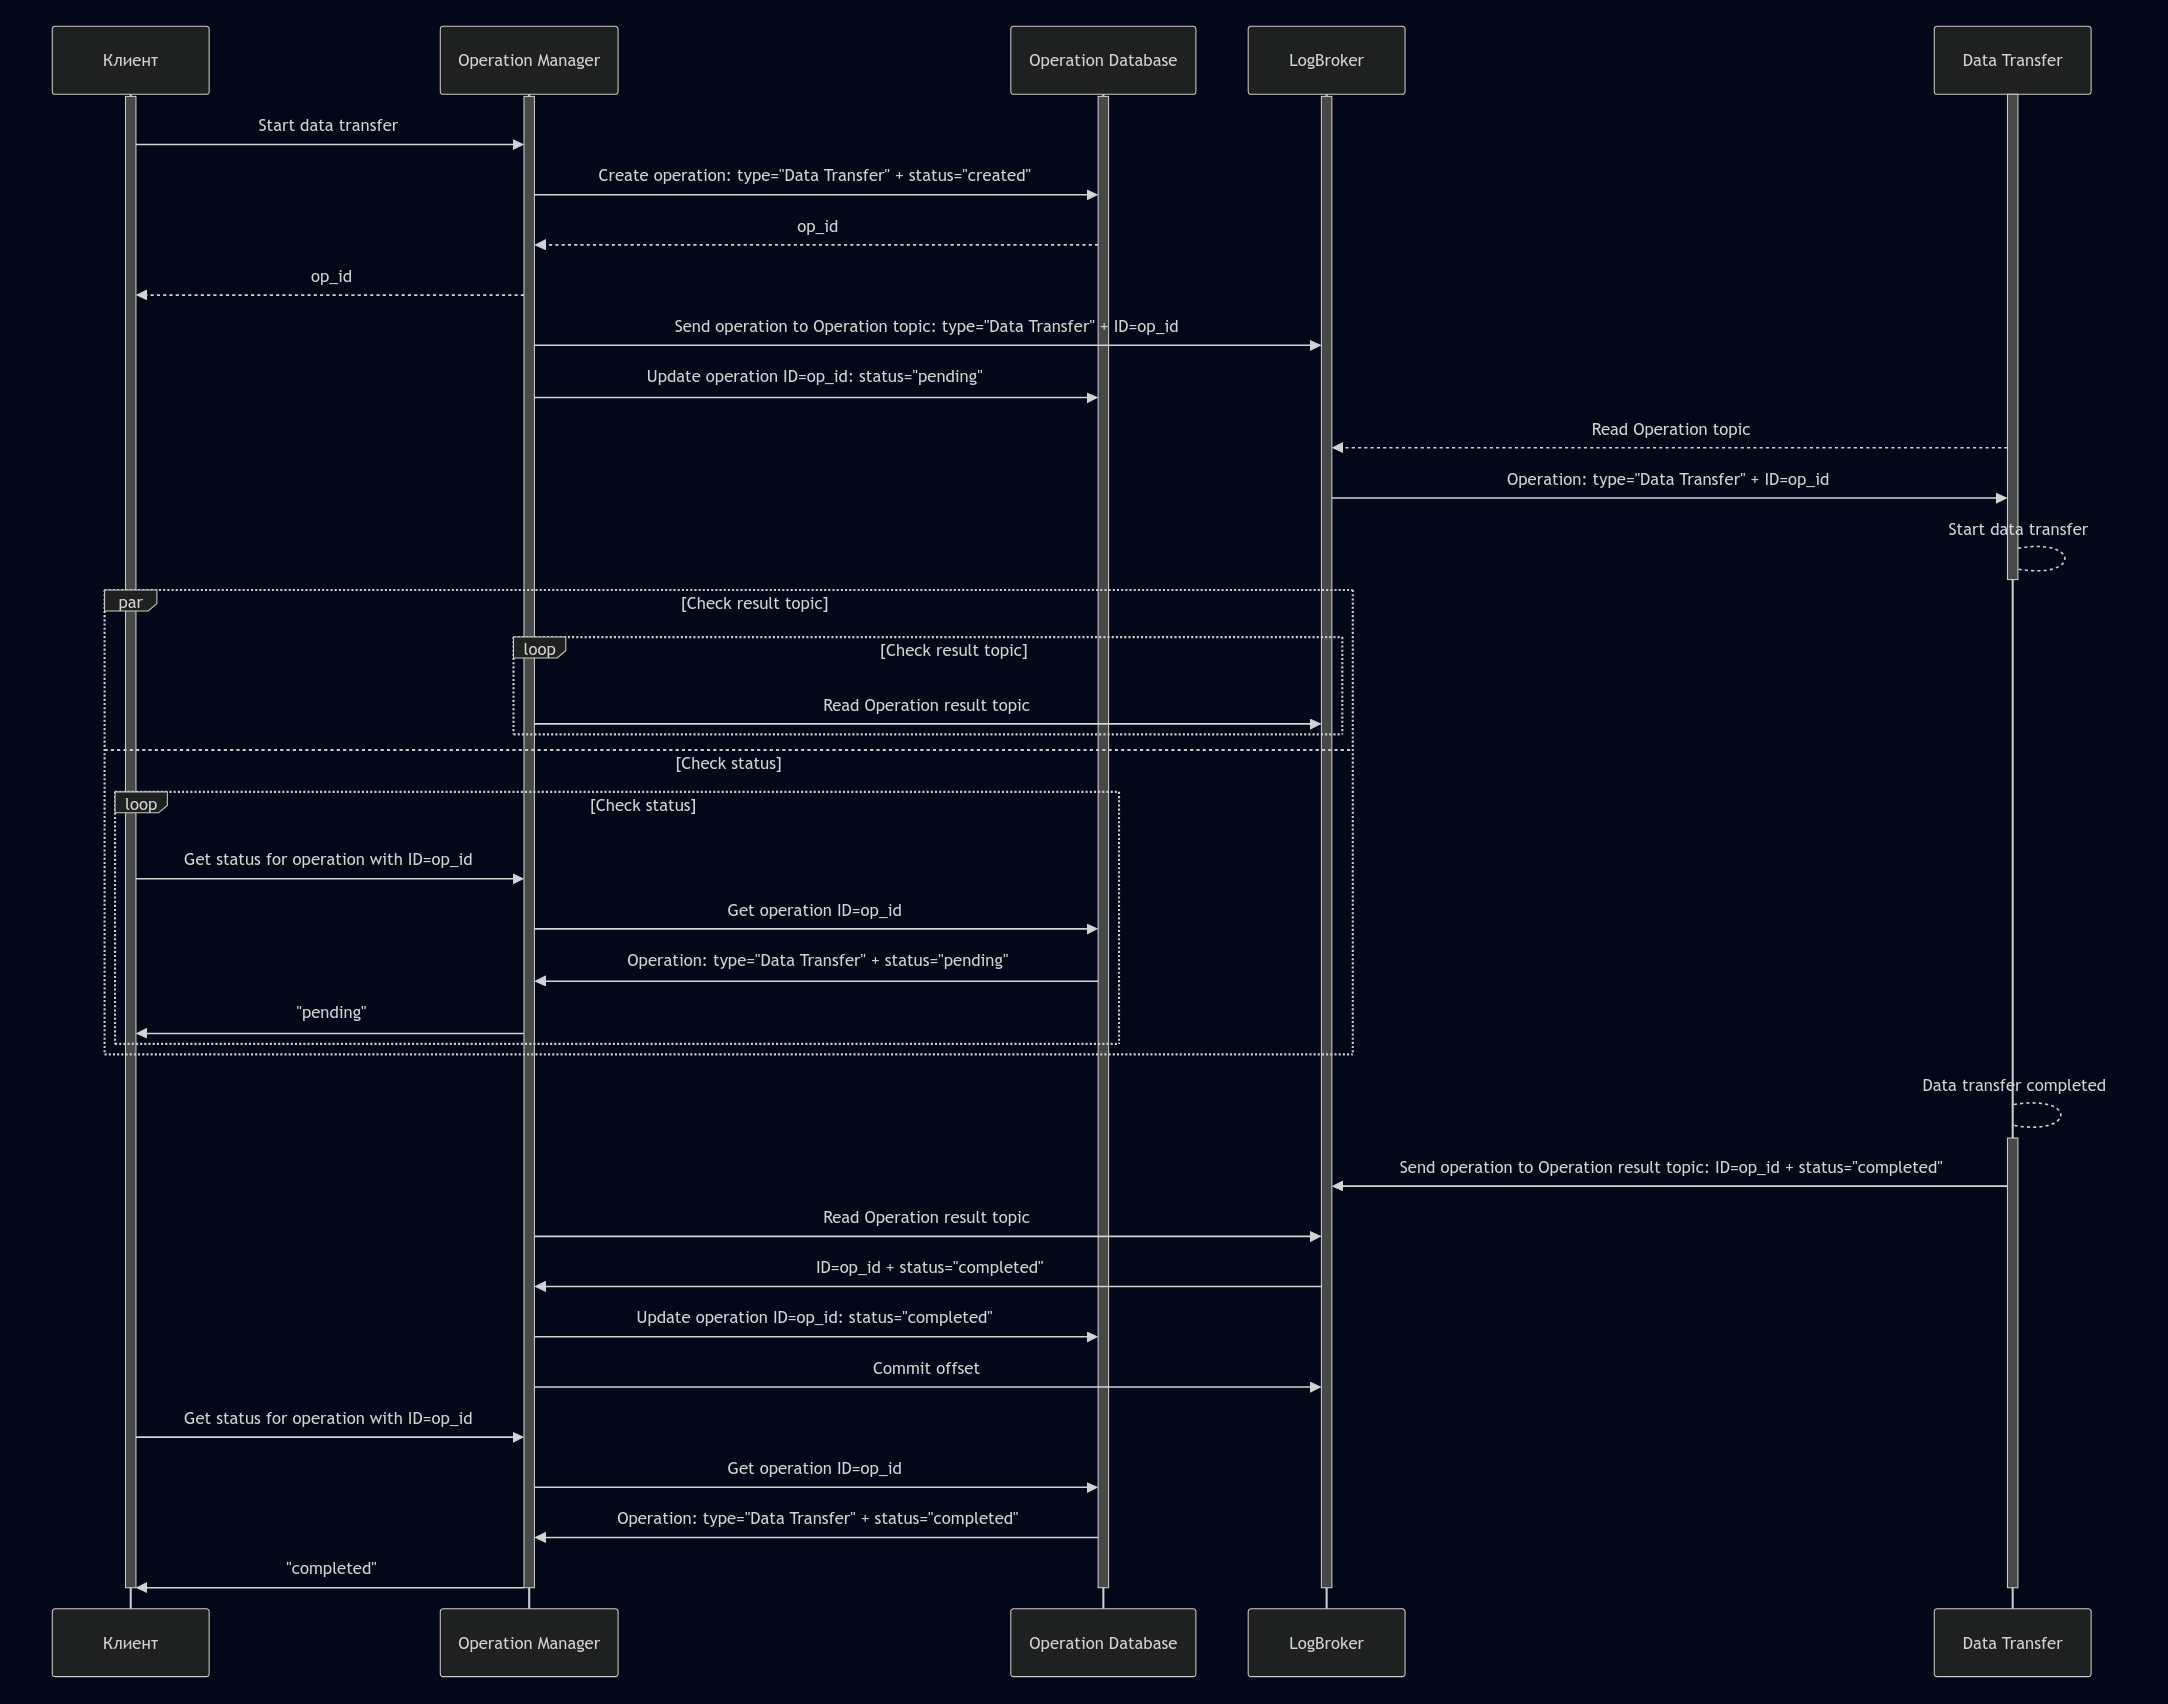
\includegraphics[scale=0.2]{./img/mermaid-sequence-User-MainSystem.png}
  \caption{Диаграмма последовательности взаимодействия пользователя с системой на примере генерации данных}
  \label{Sequence User-MainSystem}
\end{figure}

На диаграмме можно заметить, как клиент и система общаются асинхронно.

\subsubsection{Компоненты переноса данных}

\begin{figure}
  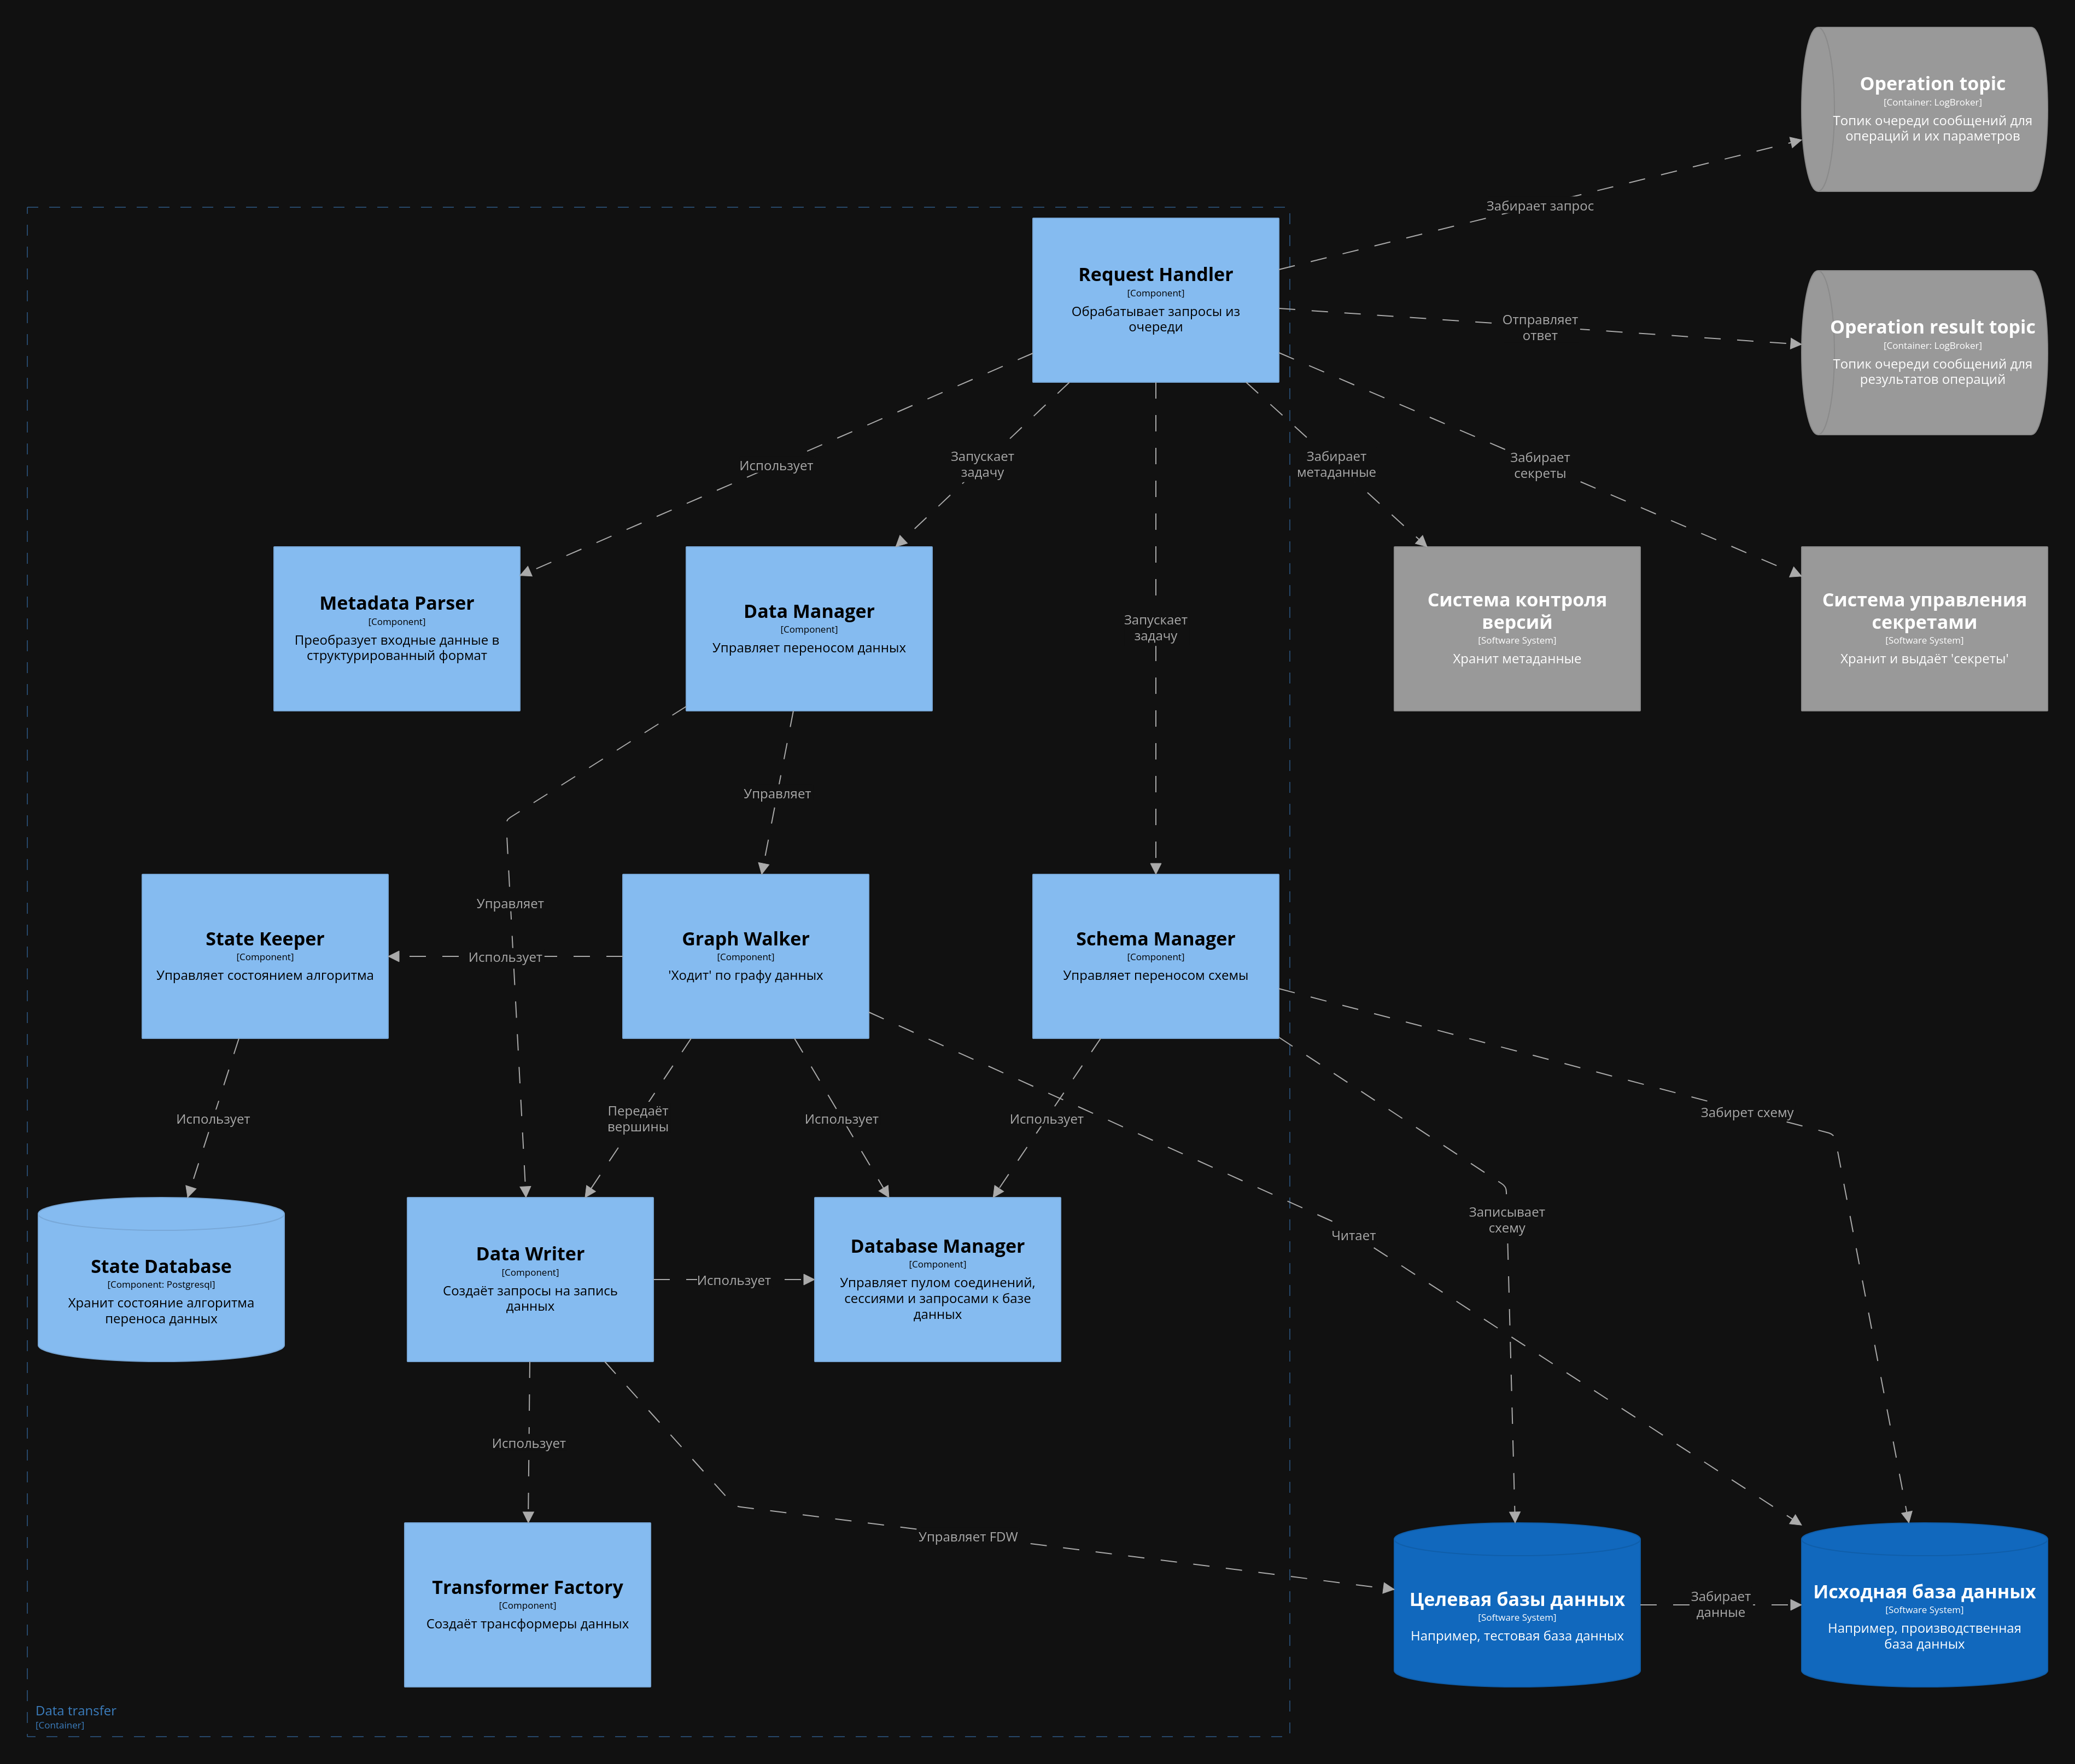
\includegraphics[scale=0.12]{./img/structurizr-DataTransferComponents.png}
  \caption{Компоненты Data Transfer}
  \label{Data Transfer Components}
\end{figure}

Рассмотрим процесс обработки запросов на перенос задач. Компонент Request Handler принимает такие запросы. Они должны включать следующие элементы:

\begin{itemize}
  \item идентификатор метаданных;
  \item идентификатор исходной базы данных;
  \item идентификатор целевой базы данных.
\end{itemize}

Идентификатор метаданных может принимать форму одной из двух сущностей: уникального идентификатора, связанного с метаданными в Системе контроля версий, или самих метаданных. В случае предоставления уникального идентификатора, Request Handler обращается к Системе контроля версий для извлечения соответствующих метаданных.

Идентификатор базы данных может быть представлен либо в форме уникального идентификатора кластера базы данных, либо в виде параметров подключения к базе данных. При предоставлении уникального идентификатора кластера базы данных, Request Handler обращается к Системе управления секретами для получения необходимых параметров подключения, включая пароль.

Полученные метаданные направляются в компонент Metadata Parser для их валидации и преобразования во внутренний формат представления. Далее инициируется Data Manager, который получает информацию о подключениях к базам данных, а также внутреннее представление метаданных, и запускает компоненты Graph Walker и Data Writer.

Компонент Graph Walker выполняет алгоритм обхода данных исходной базы, который будет рассмотрен позже, следуя инструкциям, заданным в метаданных. Он использует State Keeper для сохранения состояния алгоритма и Database Manager для выполнения операций с базой данных. В процессе работы, Graph Walker извлекает метаинформацию о посещенных вершинах и асинхронно передает её компоненту Data Writer.

Компонент Data Writer управляет преобразованием данных и их записью в целевую базу данных. Он принимает на вход метаинформацию о данных, включая их идентификаторы, и с помощью Database Manager создаёт объект Foreign Data Writer~\cite{fdw} в целевой СУБД, обеспечивая прямое подключение к исходной СУБД. Data Writer формирует запросы, включающие идентификаторы данных, направляя их в целевую СУБД для извлечения конкретных данных из исходной базы. Запросы дополняются трансформерами, сформированными на основе метаданных через компонент Transformer Factory. Трансформер представляет собой набор правил преобразования данных, например, для анонимизации данных.

Рассмотрим взаимодействие основных компонент на диаграмме последовательности.

\begin{figure}
  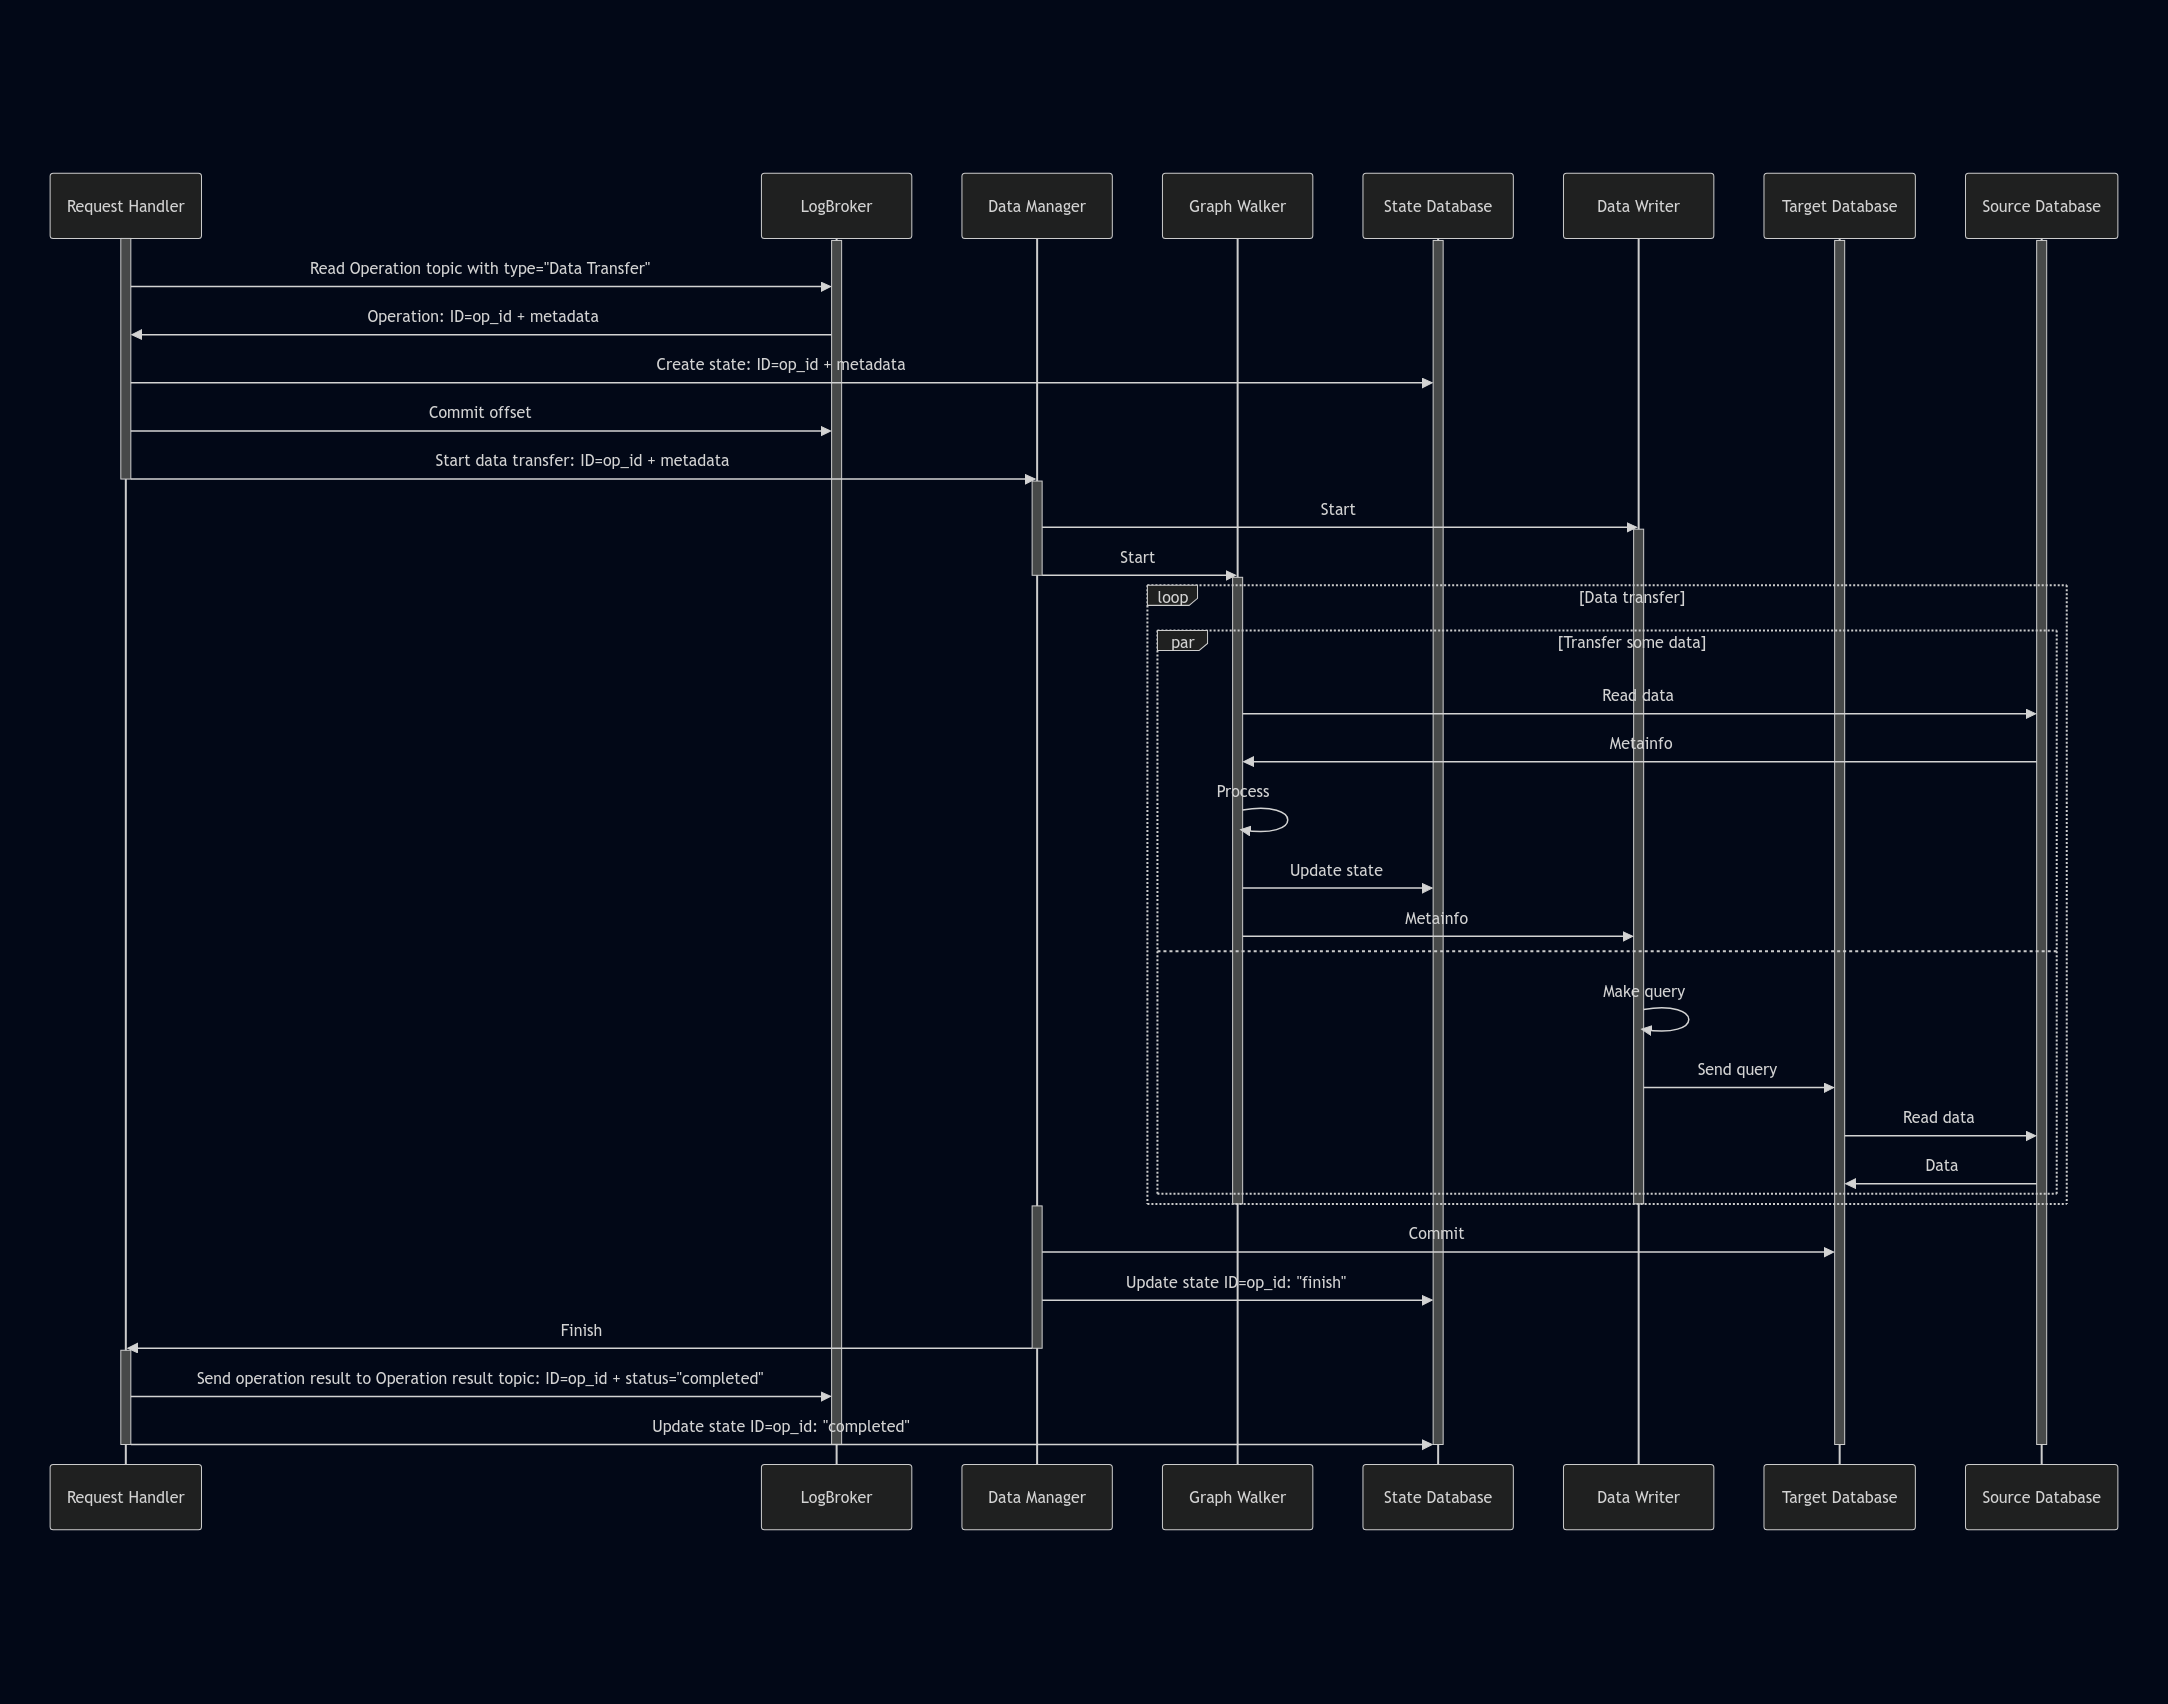
\includegraphics[scale=0.2]{./img/mermaid-sequence-DataTransfer.png}
  \caption{Диаграмма последовательности взаимодействия пользователя с системой на примере генерации данных}
  \label{Sequence DataTransferComponents}
\end{figure}

Данный подход предусматривает непосредственный перенос данных из исходной базы в целевую, с возможными изменениями в соответствии с правилами, определёнными в метаданных, что способствует повышению производительности системы.

Также на рисунке~\ref{Data Transfer Components} представлен компонент Schema Manager, который предоставляет функциональность по управлению схемами баз данных. В частности, данный компонент позволяет осуществлять перенос схемы между различными базами данных, а также выполнять удаление схемы.

\subsubsection{Компоненты генерации данных}

\begin{figure}
  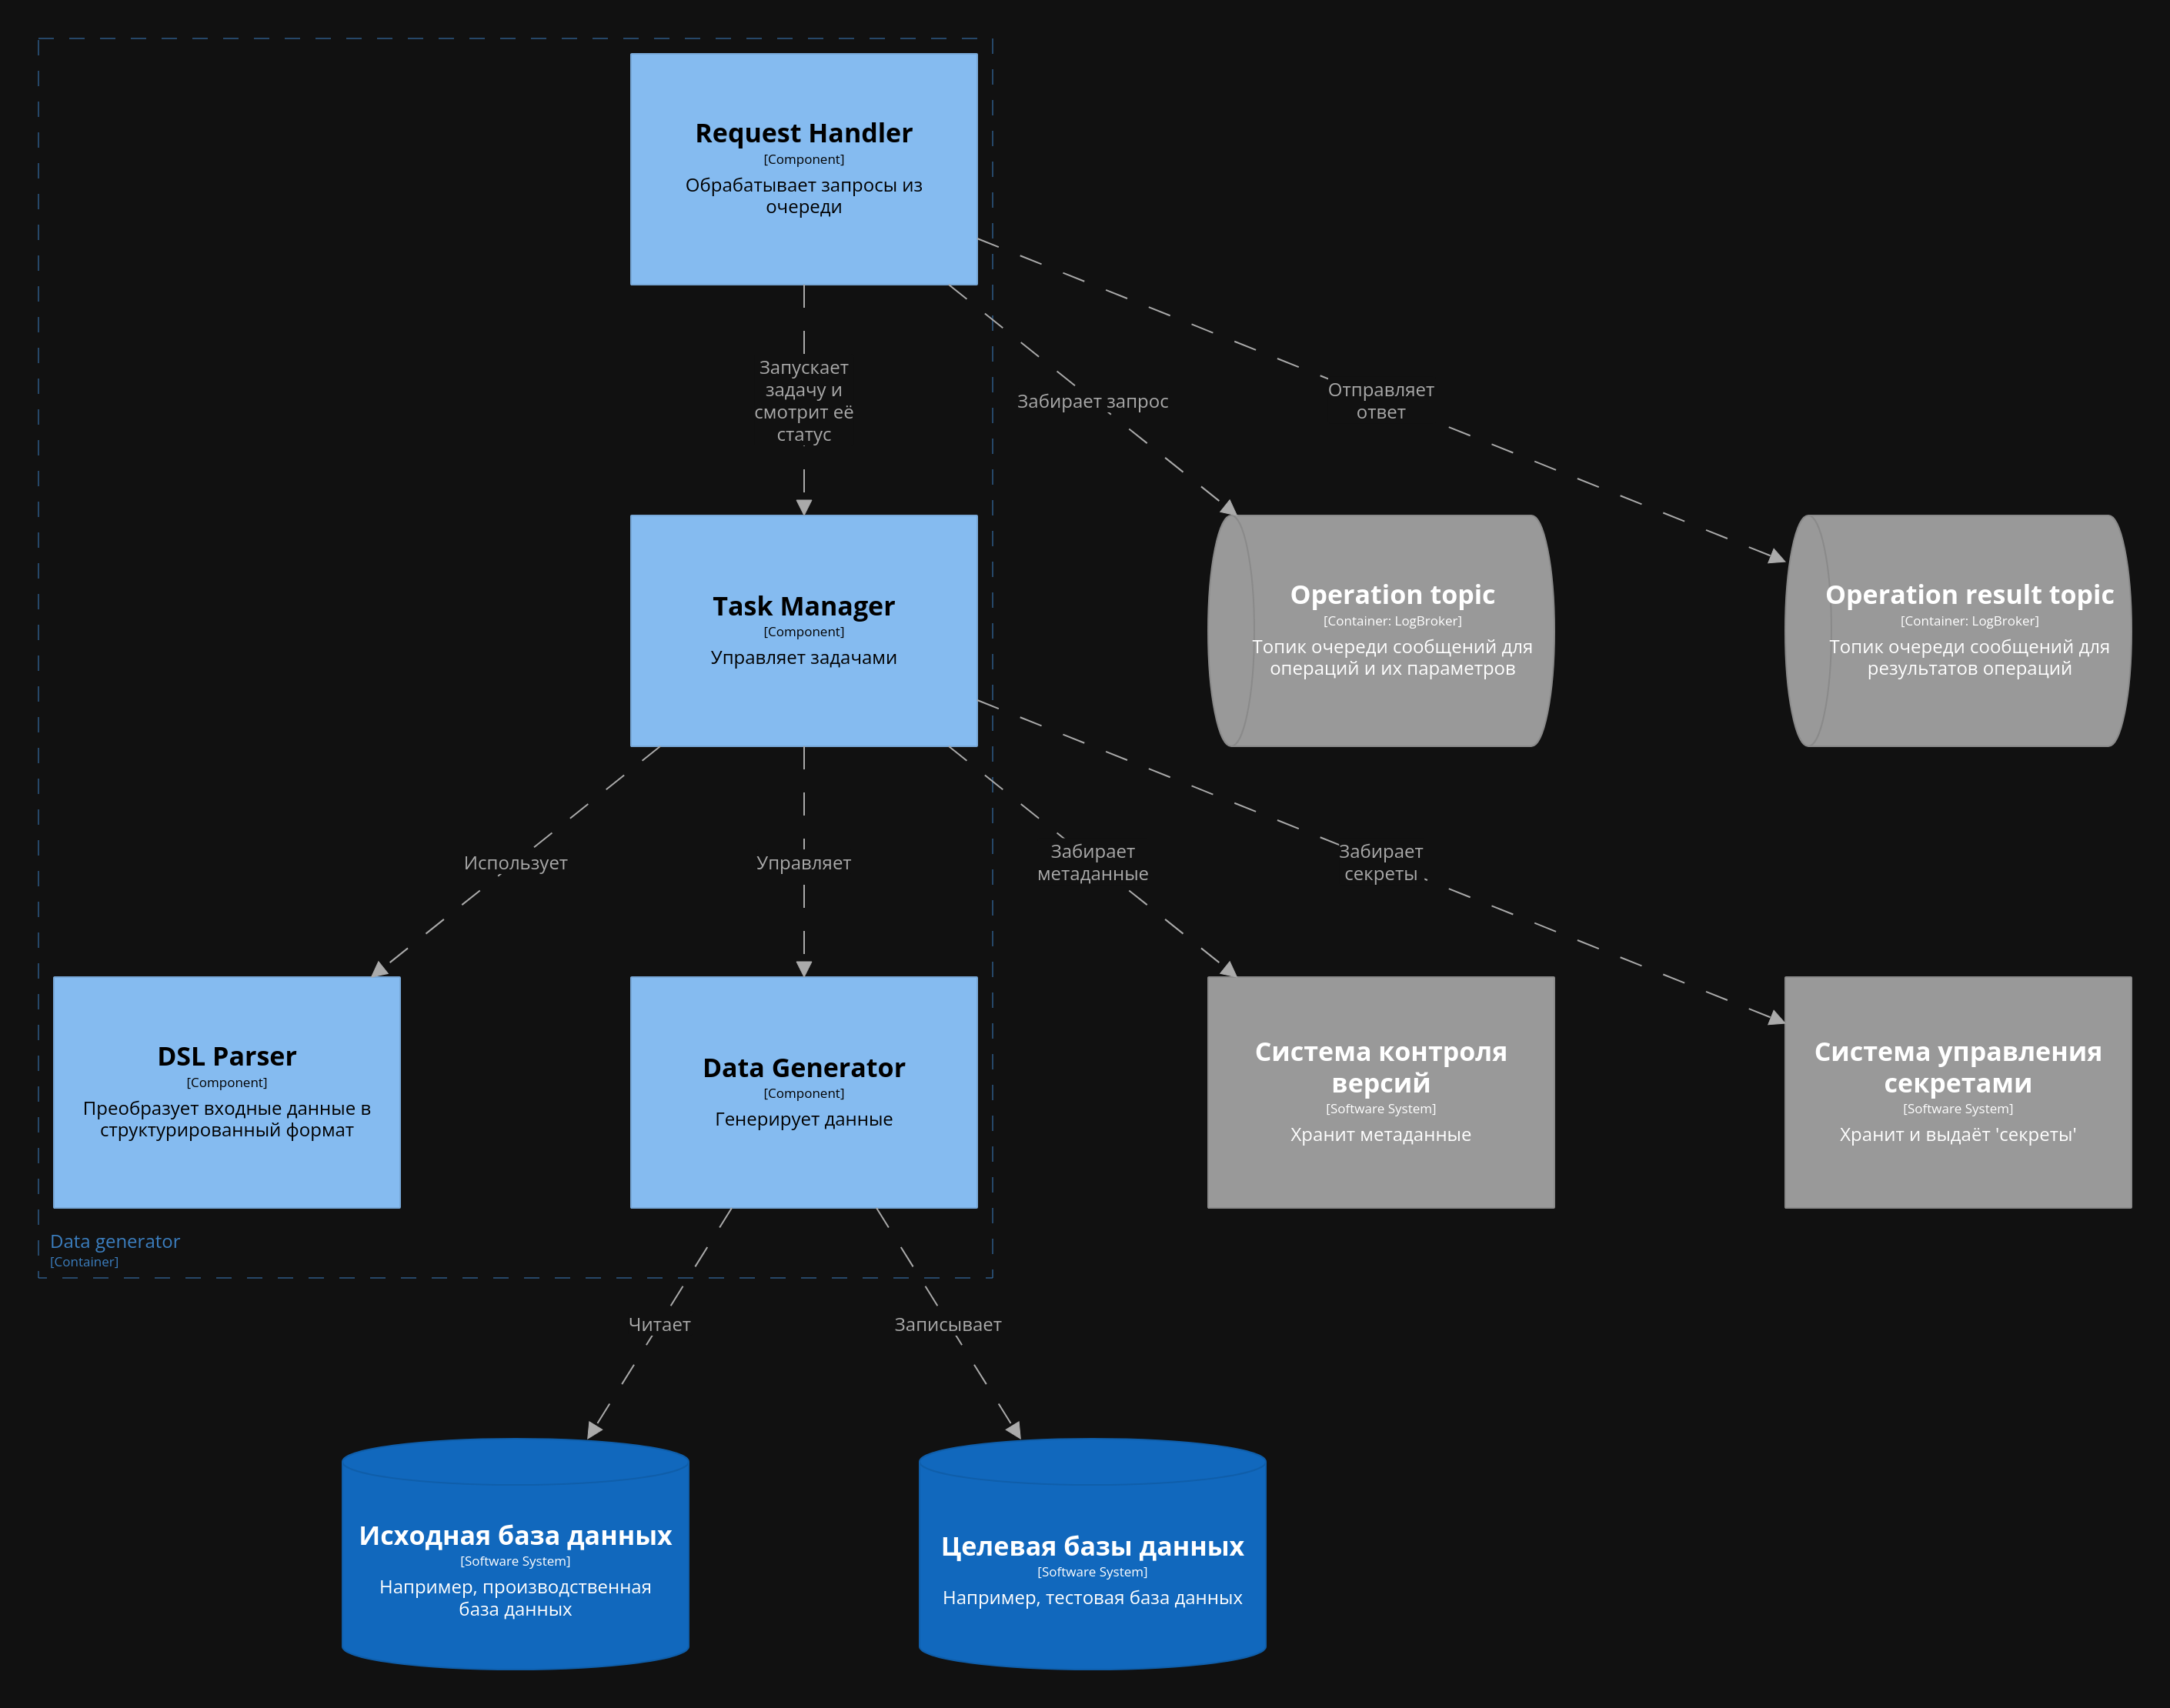
\includegraphics[scale=0.15]{./img/structurizr-DataGeneratorComponents.png}
  \caption{Компоненты Data Generator}
  \label{Data Generator Components}
\end{figure}

TBD: расписать взаимодействие компонент Data generator

\subsubsection{Персистентность состояния и восстановление после сбоя}

Процессы переноса данных могут быть времязатратными, независимо от объёма данных. В случае неожиданной остановки сервиса переноса и генерации данных, вызванной сбоем, утрата прогресса по переносу данных становится крайне нежелательным исходом.

Рассмотрим, как выполняется персистентность состояния системы, то есть её способность сохранять и восстанавливать своё состояние после остановки.

Весь процесс выполнения операции от её инициации до её завершения можно разделить на два этапа:
\begin{itemize}
  \item отправка и чтение из очереди сообщений;
  \item непосредственный процесс переноса данных.
\end{itemize}

Сбои могут возникать на любом из этих этапов. Для этапа отправки и чтения сообщений из очереди предусмотрена семантика доставки exactly-once~\cite{delivery-guarantees}, которая поддерживается использованием архитектурных паттернов Inbox Pattern и Outbox Pattern~\cite{outbox-and-inbox}. Эти паттерны, часть реализации которых можно наблюдать на диаграммах последовательностей~\ref{Sequence User-MainSystem} и~\ref{Sequence DataTransferComponents}, обеспечивают гарантированную доставку сообщений и идемпотентную обработку входящих данных.

При сбое на этапе переноса данных механизмы восстановления включают проверку состояния незавершённых операций в базе данных состояния (State Database). В ней хранится прогресс каждой операции переноса данных и включает уникальные идентификаторы операции, состояние алгоритма и метаданные. При восстановлении система переноса данных проверяет наличие незавершённых операций и продолжает их с того места, где процесс был остановлен. Запись в целевую базу данных успешно завершается только при успешном выполнении алгоритма, что требует повторной записи данных в случае восстановления после сбоя, основываясь на метаинформации из сохранённого состояния.

Таким образом, архитектура системы включает механизмы обеспечения персистентности состояния и восстановления после сбоев.

\subsubsection{Безопасность}

TBD: расписать, как выполняется свойство безопасности системы

\subsection{Алгоритм обхода данных}

Всю основную функциональность переноса данных можно разделить на две части: запись данных в целевую базу данных, которую мы рассматривали ранее, и обход исходных данных, алгоритм которого мы рассмотрим подробнее в этом разделе.

\subsubsection{Метаграфы}
TBD: рассмотрим такую структуру как метаграф. Рассказать о первоначальной идеи метаграфа и подвести к тому, что стандартного определения у метаграфа нет, поэтому мы дадим своё определение.

$MG = <V, MV, E, ME>$ -- метаграф, где $V$ -- множество вершин, $MV$ -- множество метавершин, $E$ -- множество рёбер, $ME$ -- множество метарёбер.

$v_i = \{atr_k\}, v_i \in V$, где $v_i$ -- вершина, $atr_k$ -- атрибут.

$mv_i = <\{v_j\}, \{atr_k\}>, mv_i \in MV, v_j \in V$, где $mv_i$ -- метавершина, $v_j$ -- вершина, $atr_k$ -- атрибут.

$e_i = <v_s, v_e>, e_i \in E, v_s, v_e \in V$, где $e_i$ -- ребро, $v_s$ -- исходная вершина, $v_e$ -- конечная вершина.
$me_i = <mv_s, mv_e, \{atr_k\}>, me_i \in ME, mv_s, mv_e \in MV$, где $me_i$ -- метаребро, $mv_s$ -- исходная метавершина, $mv_e$ -- конечная метавершина, $atr_k$ -- атрибут.

Также введём ограничение на множество метавершин: $\forall mv_i, mv_j \in V, i \neq j => \{v_x\}_i \cap \{v_y\}_j = \emptyset$, т.е. каждая вершина не может содержаться в нескольких метавершинах.

\subsubsection{Представление базы данных в виде метаграфа}

TBD: расписать эту секцию получше

Для реляционной базы данных метаграф это:
\begin{itemize}
  \item вершины обозначают данные; атрибуты -- полезная нагрузка;
  \item метавершины обозначают таблицы, содержащие данные; атрибуты -- структура таблицы;
  \item рёбра показывают, как связаны данные;
  \item метарёбра показывают, как связаны таблицы (по Foreign Key); атрибуты -- названия полей, по которым связаны таблицы.
\end{itemize}

\subsubsection{Описание алгоритма}
TBD: здесь хочу описать общий алгоритм, не привязываясь к конкретным СУБД

\begin{figure}
  \fontsize{12pt}{14pt}\selectfont
  \begin{lstlisting}
// TBD: написать алгоритм
BFSforMetagraph(graph, startVertex)
   // Инициализация
   queue := {}
   visited := {}
  \end{lstlisting}
  \caption{Алгоритм }
\end{figure}

\subsubsection{Устройство Postgresql}
TBD: здесь хочу описать некоторые моменты из устройства Postgresql: ctid, tableoid -- они применяются в имплементации алгоритма.

\subsubsection{Имплементация}
TBD: здесь хочу наложить алгоритм на Postgresql и написать имплементацию алгоритма на Python (которая уже готова, но её просто так нельзя выкладывать :D).

\subsection{Генерация данных}
TBD: генерация данных далеко не основная функциональность системы, поэтому времени ей будет уделено немного

\subsection{Разработка языка}
TBD: есть синтаксис языка, но нужно реализовать парсер. Структура этого раздела пока под вопросом

\subsubsection{Синтаксис и грамматика языка}

\subsubsection{Корректность языка}

\subsubsection{Язык задания графа}

\subsubsection{Язык переноса данных}

\subsubsection{Язык генерации данных}

\section{Демонстрация программного продукта и анализ результатов}

\subsection{Обзор прототипа}
В рамках дипломной работы был разработан прототип системы в виде инструмента c интерфейсом командной строки. Рассмотрим его функциональность.

Прототип обеспечивает перенос данных и их удаление из базы данных. Кроме того, данный инструмент позволяет осуществлять перенос и удаление схемы базы данных или выводить схему в формате диаграммы PlantUML \cite{plantuml}.

В прототипе реализованы основные компоненты, указанные в \ref{Sequence DataTransferComponents}, включая элементы Graph Walker и Data Writer. Процесс обхода данных основан на алгоритме \ref{algorithm-with-rules}. Для записи данных из одной базы в другую применяется механизм Foreign Data Wrapper.

Кроме того, в прототипе предусмотрены две версии взаимодействия с базой данных и между компонентами Graph Walker и Data Writer: синхронная и асинхронная. В случае синхронного взаимодействия компонент Graph Walker ожидает завершения записи данных компонентом Data Writer, в то время как при асинхронном взаимодействии компоненты функционируют независимо друг от друга.

Также в прототипе поддерживается функциональность следующих конструкции для описания метаданных: \textit{GRAPH SOURCE}, \textit{NO ENTER}, \textit{NO EXIT}, \textit{LIMIT DISTANCE}.

\subsection{Примеры использования и производительность}

TBD: описать какой-нибудь пример с бд, описанной ранее.

TBD: наполнить базку множеством данных и потестить прототип на ней. Можно сравнить производительность синхронной и асинхронной версий, а также использовать pg\_dump

\subsection{Анализ результатов}

TBD: сделать анализ получившегося прототипа. Написать про жизнеспособность системы: можно ли пользоваться этой системой, либо проще использовать готовые инструменты, в том числе обычные SQL-запросы.


\conclusion

В ходе дипломной работы была спроектирована система переноса и генерации взаимосвязанных данных. Были детально описаны алгоритмы выбора и генерации взаимосвязанных данных, разработан специфальный язык для описания метаданных, а также создан прототип системы. Дополнительно проведено тестирование производительности прототипа и осуществлён анализ жизнеспособности системы.

Несмотря на то, что проектирование и разработка проводились при тестировании образовательной платформы и основное тестирование прототипа осуществлялось с использованием одной базы данных, предлагаемая система обладает универсальностью и может быть интегрирована в другие платформы и применена в различных областях. Важным аспектом архитектуры системы является то, что функции, характерные для работы с PostgreSQL, инкапсулированы в одном компоненте. Это способствует легкой адаптации системы к другим реляционным СУБД.

В процессе разработки и тестирования прототипа были выявлены места, требующих улучшения:
\begin{itemize}
    \item первая проблема заключается в возникновении сложностей в понимании структуры базы данных и алгоритма обхода, что делает трудоёмким написание метаданных, которые бы удовлетворяли потребности пользователя. Возможным решением этой проблемы может стать создание инструмента для анализа структуры базы данных, аналогичного Jailer, который бы поддерживал описанный алгоритм обхода и правила метаграфа. Предполагаемый инструмент обеспечит пользователю возможность эффективной визуализации структуры базы данных и упростит процесс описания правил метаграфа;
    \item вторая проблема заключается в низкой производительности программы, особенно при больших объёмах данных. Есть гипотеза, что низкая производительность связана с частыми сетевыми запросами в базы данных. В качестве потенциального решения данной проблемы предлагается модификация взаимодействия с базой данных путём замены множественных мелких запросов на более редкие, но масштабные обращения к данным.
\end{itemize}
 % Заключение

\printbibliography % Список литературы

\appendix % Приложения
\appendixsection{Исходный код грамматики на ANTLR4}

На рисунке \ref{qr-lang} изображён QR-код со ссылкой на GitHub репозиторий с исходным кодом разработанной грамматики языка на ANTLR4.

\begin{figure}
  
\includegraphics[scale=0.5]{./img/qr-code-relatio-lang.png}
  \caption{QR-код на репозиторий c грамматикой}
  \label{qr-lang}
\end{figure}

\end{document}
